\section{Concept E: Kinetic Bolas}

The initial design phase explored three tether-based recovery concepts for balloon-borne payloads: the Payload-Hover Drone, where the UAS attaches directly to the payload; the Collaborative Tether, involving a dual-drone team; and the Kinetic Bolas Wrap, utilizing a weighted projectile to create a high-friction anchor. A trade-off analysis, presented in \autoref{tab:drone_power_analysis}, evaluated power consumption and battery mass across these configurations for both Multirotor (Quad) and VTOL platforms. The Tethered Drone and Collaborative Tether concepts were disqualified due to prohibitive power requirements and operational complexity, respectively, leading to the selection of the Kinetic Bolas concept.

\begin{table}[H]
\centering
\caption{Comparative Analysis of Power Requirements and Battery Mass}
\label{tab:drone_power_analysis}
\begin{tabular}{lrrrrr}
\toprule
\textbf{Flight Metric} & \textbf{Bolas Quad} & \textbf{Bolas VTOL} & \textbf{Hover Quad} & \textbf{Hover VTOL} & \textbf{Tethered Drone} \\
\midrule
Hover Power (W)    & 2,881.65  & 4,075.26  & 6,830.57  & 9,659.88  & 23,053.17 \\
Climb Power (W)    & 7,296.15  & 5,699.14  & 15,659.57 & 5,794.75  & 40,711.17 \\
Cruise Power (W)  & 7,139.93  & 2,358.03  & 7,449.28  & 2,652.78  & 23,671.88 \\
Descent Power (W) & 17,842.01 & 17,842.01 & 18,350.96 & 19,781.72 & 23,053.17 \\
\midrule
Total Energy (kJ)  & 25,584    & 22,115    & 32,430    & 25,770    & 66,294    \\
Battery Mass (kg) & 40.38     & 34.90     & 51.18     & 40.67     & 104.63    \\
\bottomrule
\end{tabular}
\end{table}

\subsection{System Architecture}
\label{subsec:concept_A_architecture}
The system architecture has been established at a conceptual level. Each subsystem is discussed below and is visually represented by the conceptual impression in \autoref{fig:concept_e_ai}.

\begin{figure}[H]
     \centering
     \begin{subfigure}[b]{0.48\textwidth}
         \centering
         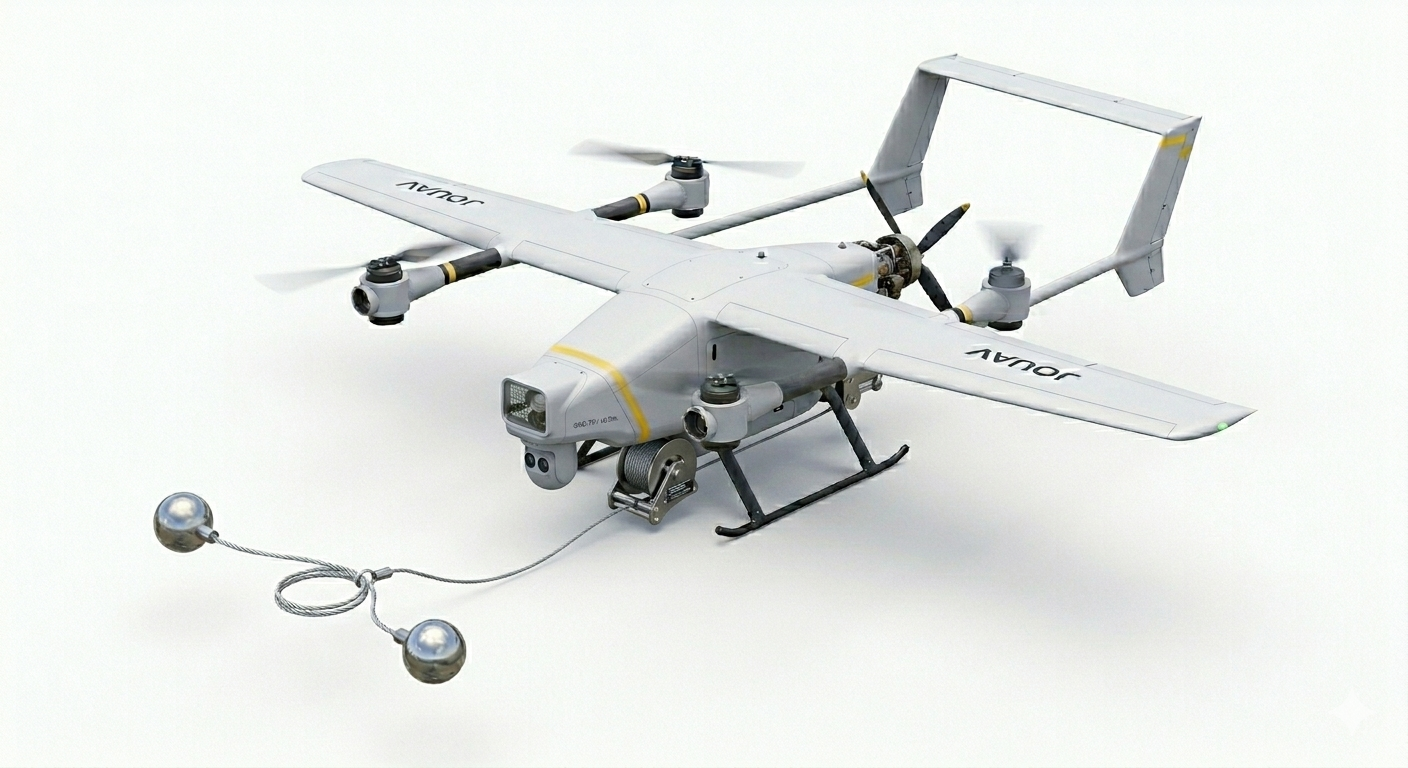
\includegraphics[width=\textwidth]{figures/Gemini_Generated_Image_9h0fwa9h0fwa9h0f.png}
         \caption{Initial impression}
         \label{fig:concept_e_ai}
     \end{subfigure}
     \hfill
     \begin{subfigure}[b]{0.25\textwidth}
         \centering
         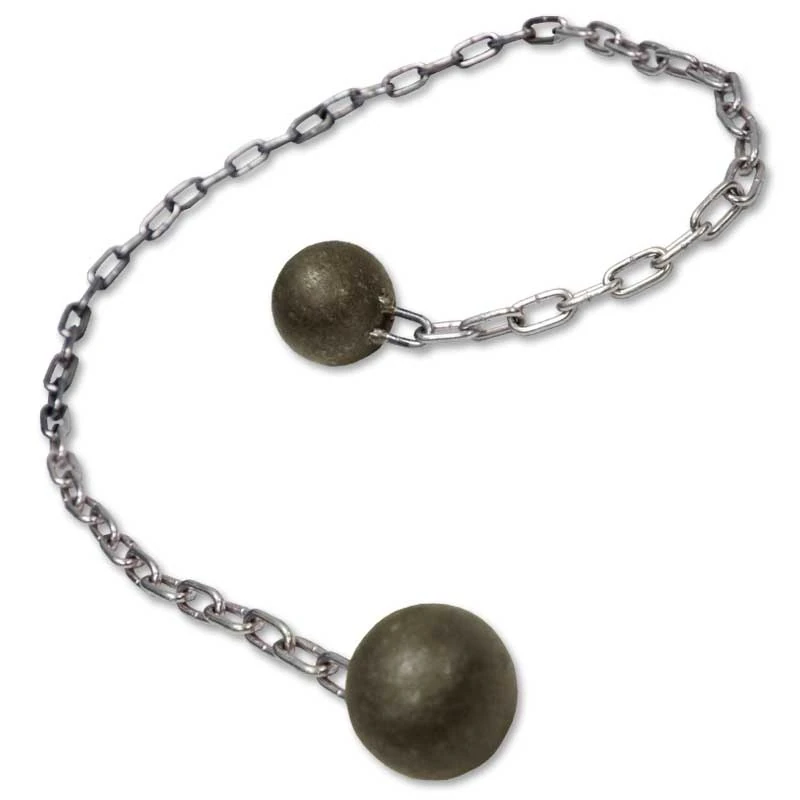
\includegraphics[width=\textwidth]{figures/Concepts/Bolas.png}
         \caption{Bola example}
         \label{fig:placeholder}
     \end{subfigure}
     \caption{Comparison of initial concept and reference example.}
     \label{fig:combined_comparison}
\end{figure}
\todo{i dont really like the bola example but idk what else to put}

\subsubsection{Aerial Platform}
A lift-and-cruise hybrid configuration was selected for the conceptual design. This architecture provides high-efficiency forward flight necessary for long-range transit while maintaining a stable, high-accuracy hover platform required to aim and fire the bolas mechanism. This configuration avoids the control instabilities inherent in tailsitter designs during the high-precision shooting phase and enables the use of a unified sensor suite for both flight modes.

\subsubsection{Sensing and Tracking}
The sensing suite for this concept is similar to that described in \autoref{subsec:Sensing_tracking}.\todo{not Figure, but Section} The primary challenge involves maintaining a stable hover next to the balloon for bola deployment, requiring relative position maintenance with sub-meter precision (target < 0.5 m). Given the chosen aerial platform, a single sensor suite placed in the nose of the drone is sufficient. Additionally, a tether tension sensor is integrated to prevent overstressing the suspension lines.

\subsubsection{Balloon Interaction Mechanism}
The UAS utilizes a pneumatic launcher to fire a bola, two weighted projectiles connected by a high-strength leader line. These weights are discharged from the engine pods to ensure a separation of more than one meter, providing additional margin for positioning accuracy. Upon impact with the vertical suspension lines, the projectiles' momentum causes them to wrap around the target. This utilizes the Capstan Effect, where friction increases exponentially with each wrap, securing the anchor point without mechanical clamps. The UAS monitors attachment via tension sensors; if attachment is insufficient, the drone performs orbiting maneuvers to increase wrap count.

\subsubsection{Descent Initiation}
Once the bolas has entangled the vertical line, the UAS transitions to a descent profile. The aircraft moves away from the balloon while reeling out its tow line, utilizing both its mass and directed thrust from the VTOL and cruise motors to manage the balloon's trajectory toward the designated recovery site.

\subsubsection{Descent Management and Recovery}
During descent, the UAS requires minimal vertical thrust, as it is primarily supported by the balloon in a pendulum-like configuration. If horizontal corrections are necessary, thrust is generated to steer the balloon toward the target zone.

\subsubsection{Ground Segment and Operator Role}
Ground support requirements are divided into personnel for reloading expendables and the maintenance of the ground link required for detection and monitoring.

\subsection{Mass, Cost, and Power Estimates}
The initial mass estimate incorporates mass fractions, margins, and the allocation for the pneumatic bolas launcher, as shown in \autoref{tab:mass_fractions_bolas}.

\begin{table}[htbp]
\centering
\caption{Mass Fractions and Component Weights}
\label{tab:mass_fractions_bolas}
\begin{tabular}{lcccc}
\toprule
\textbf{Parameter} & Structure Fraction & Propulsion Fraction & Avionics Fraction & Launcher Weight (kg) \\
\midrule
\textbf{Value} & 0.27 & 0.27 & 0.05 & 3.75 \\
\bottomrule
\end{tabular}
\end{table}

Using the power-based mass iteration described in \autoref{sec:power_mass}, the power requirements and final mass distribution for the Lift+Cruise architecture were determined. These results are summarized in \autoref{tab:lift_cruise_power} and \autoref{tab:lift_cruise_weight}.

\begin{table}[H]
    \centering
    \begin{minipage}{0.48\textwidth}
        \centering
        \caption{Power and Energy Requirements}
        \label{tab:lift_cruise_power}
        \small
        \begin{tabular}{lr}
            \toprule
            \textbf{Parameter} & \textbf{Value} \\
            \midrule
            Hover power (W)    & 3,490.79 \\
            Cruise power (W)   & 754.22   \\
            Climb power (W)    & 5,174.05 \\
            Descent power (W)  & 4,000.00 \\
            \midrule
            Total energy (J)   & 7,004,195.17 \\
            Battery mass (kg)  & 11.05    \\
            \bottomrule
        \end{tabular}
    \end{minipage}
    \hfill 
    \begin{minipage}{0.48\textwidth}
        \centering
        \caption{Mass Breakdown}
        \label{tab:lift_cruise_weight}
        \small
        \begin{tabular}{lr}
            \toprule
            \textbf{Component} & \textbf{Mass [kg]} \\
            \midrule
            Structure \& frame  & 10.18 \\
            Propulsion          & 10.18 \\
            Avionics            & 1.88  \\
            Capture mechanism    & 3.75  \\
            Battery             & 11.05 \\
            Margin (10\%)       & 0.65  \\
            \midrule
            \textbf{ESTIMATED MTOW} & \textbf{37.69} \\
            \bottomrule
        \end{tabular}
    \end{minipage}
\end{table}

This initial estimate is corroborated by a review of off-the-shelf components, which also serves as the basis for cost estimation. A detailed breakdown is provided in \autoref{tab:component_breakdown}.

\begin{table}[H]
    \centering
    \caption{Component Mass, Cost and Source Breakdown for Lift+Cruise UAS}
    \label{tab:component_breakdown}
    \small
    \setlength{\tabcolsep}{4pt}
    \renewcommand{\arraystretch}{1.15}
    \begin{tabularx}{\textwidth}{@{}XrrX@{}}
        \toprule
        \textbf{Component} & \textbf{Cost [EUR]} & \textbf{Mass [kg]} & \textbf{Source basis} \\
        \midrule
        Battery system & 2,819.94 & 14.760 & \cite{TattuGmbH} \\
        Lift motors & 1,519.60 & 3.960 & \cite{U13Drones} \\
        Lift ESCs & 679.96 & 1.438 & \cite{ALPHAStability} \\
        Lift propellers & 715.80 & 0.428 & \cite{G3211Store} \\
        Cruise motor & 229.00 & 0.780 & \cite{AT7224Smooth} \\
        Cruise ESC & 109.99 & 0.182 & \cite{T-MOTORController} \\
        Cruise propeller & 118.90 & 0.080 & \cite{AUZPropeller} \\
        Airframe structure & 2,000.00 & 7.900 & \cite{CarbonCompositesb,CarbonComposites,Aluminum7075-T651,CuredComposites} \\
        Avionics suite & 973.97 & 0.659 & \cite{PixhawkStore,DroneCANStore,SiKStore,PM08-CANStore,AS150Amass,FLYRCGames,AlleDrones} \\
        Bolas \& reel mechanism & 1,415.00 & 3.750 & \cite{GummiuberzogeneOse,D12Ltd,MarlowPB,UmarexPatronen,UmarexAccessoires,ASAZ-RAM.net,16mmComposites,RSRS,HS-5085MGRCD,CuredComposites} \\
        Hardware \& wiring & 400.00 & 1.200 & \cite{AS150Amass,FLYRCGames,AlleDrones,CuredComposites} \\
        \midrule
        \textbf{Total} & \textbf{10,982.16} & \textbf{35.137} & -- \\
        \bottomrule
    \end{tabularx}
\end{table}
\todo{ADD MARGIN FOR SENSORS TO MASS AND COST}
\subsection*{Size Estimate}
The design leads to an initial weight estimate of approximately 37.3 kg. Sizing drivers include propeller diameter and wingspan. With a vertical propeller radius of 0.7 m, a horizontal propeller radius of 0.4 m, and a chord $c = 0.7$ m, the longitudinal extension is:
\begin{equation}
    L_x = 4 \cdot R_{VTOL} + 2 \cdot R_{FWD} = 2.4\,\text{m}
\end{equation}
Given a wing surface of 5.4 m$^2$, the resulting wingspan is 7.7 m. Consequently, the total footprint is $7.7\,\text{m} \times 2.5\,\text{m}$. An initial layout is illustrated in \autoref{fig:lift_and_cruise}.

\begin{figure}[H]
    \centering
    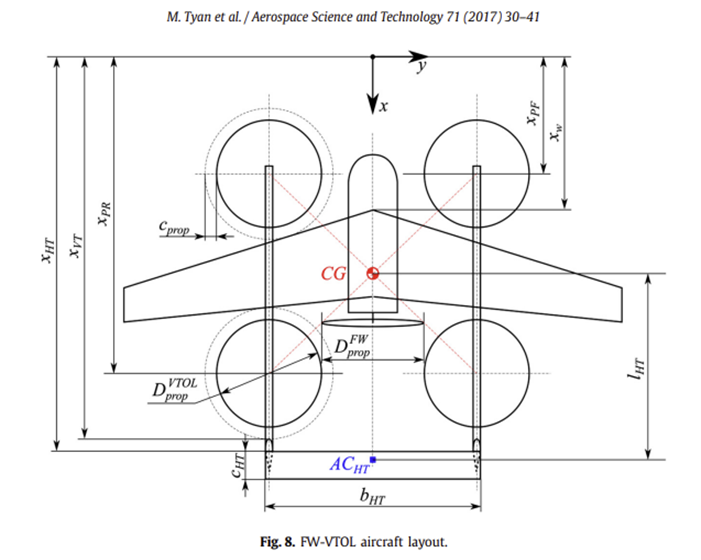
\includegraphics[width=0.7\linewidth]{figures/Concepts/lift_and_cruise.png}
    \caption{Lift-and-cruise UAS architecture selected for the recovery mission.}
    \label{fig:lift_and_cruise}
\end{figure}

\subsection{Risks and Uncertainties}
Operational risks for the Kinetic Bolas concept center on the ballistic accuracy of the pneumatic system and the mechanical reliability of the Capstan Effect.

\begin{table}[H]
\centering
\small
\caption{Key risks and mitigation strategies for the Kinetic Bolas concept.}
\label{tab:conceptE_key_risks}
\begin{tabularx}{\textwidth}{p{0.27\textwidth} X p{0.30\textwidth}}
\toprule
\textbf{Risk} & \textbf{Effect on mission} & \textbf{Possible mitigation} \\
\midrule
Ballistic Miss & The bolas fails to wrap around the line, leading to mission failure. & Include multiple bolas for redundancy. \\
Capstan Effect Failure & Insufficient wrapping results in the bolas sliding down the tether. & Use tension sensors to trigger active orbiting maneuvers to increase wrap count. \\
Tether Overstress & Dynamic loads exceed line safety factor (SF = 2.25), causing a snap. & Real-time load monitoring and active thrust control to reduce stress peaks. \\
Propeller Entanglement & The line enters the rotor disk during transition. & Use protective shrouds or electronic line-cutters; maintain standoff distance. \\
\bottomrule
\end{tabularx}
\end{table}


\subsection*{Summary and Conclusions: Concept E}


The kinetic bolas concept serves as a tether-based recovery system for balloon-borne payloads, utilizing a pneumatic launcher to discharge weighted projectiles connected by a high-strength leader line. This mechanism exploits the capstan effect, where the momentum of the projectiles causes the line to wrap around target suspension lines, creating a high-friction anchor point without mechanical clamping.

The system is integrated into a lift and cruise hybrid aerial platform, which provides the necessary high-efficiency forward flight for transit and the stable hover capability required for sub-meter positioning accuracy during engagement. Once the bolas is secured, the aircraft transitions into a managed descent profile, using directed thrust to guide the balloon toward a recovery site.

This design was concluded to be the most viable option among the studied tethered concepts due to its superior energy efficiency. While other tethered designs required excessive battery mass, the kinetic bolas configuration results in a total estimated mass of 37.69 kg and a battery mass of 11.05 kg. Cost analysis based on off-the-shelf components places the system expenditure at approximately 10,982 EUR. Although risks such as ballistic accuracy and line entanglement were identified, they are mitigated through the use of redundant projectiles, tension sensors, and active orbiting maneuvers.